\newpage 
\subsection{Elektromagnet-kraftmåling}\label{bilag_elektromagnet}
\subsubsection*{Formål}
Formålet med denne journal er at undersøge muligheden for en elektromagnet til at holde bilen på banen i svingene. For at opnå bedst mulige omgangs tid, bør elektromagnet undersøges for om man kan lave en effektiv løsning til at fastholde bilen, så den ikke skrider i sving, med max hastighed. Der laves en prøve magnet, der har pasform til at kunne placeres under bilen. Samtidig skal der testes for hvor meget kræften falder med i forhold til afstand mellem magneten og skinnerne. Derudover testes permanent magneten for hvor stærk den er og sammenlignes herefter med elektromagneten.\\
\\
\subsubsection*{Materiale liste}
\begin{itemize}
	\item Materiale af stål
	\item Kobbertråd af 0.25 mm
	\item Strømforsyning
	\item Pasco Force sensor
	\item Bilens permanent magnet
	\item Magnetisk metal plade
	\item Papir af 0.2 mm tykkelse
	\item Program, PASCO capstone
	\item Computer
\end{itemize}
 
\subsubsection*{Opstilling}
\begin{enumerate}
	\item Der skæres og slibes en magnet af ferromagnetisk materiale 
	\item Der vikles vindinger rund om magneten indtil en bredde på 4 mm er ca. opfyldt, da der er 6 mm bilens undervogn til skinnerne, skal der opnås en måling på 2 mm luftgab.
	\item Force sensoren placeres så den kan måle magnetens kraft når den trækkes af, en metal plade 
	\item En computer med programmet PASCO capstone som kan læse kraft målingerne.
 \end{enumerate}

\subsubsection*{Forsøgs beskrivelse}
Forsøget går ud på at lave en elektromagnet der kan sidde under bilen, derfor laves en test magnet af 660 vindinger da der ikke kan være så flere vindinger. En kraftmåler opstilles så den kan måle begge elektromagneters ender, der sættes 14 V over elektromagneten og kraften måles nu ved at trække elektromagneten af kraftmåleren. Forsøget gentages nu med et stykke papir på 0,2 mm, dernæst 0,4 mm, indtil vi når op på 2mm. Permanentmagneten testes, den sættes på kraftmåleren og der trækkes ned af, hvor målingerne nu er gemt på computeren.

\subsubsection*{Data}
De nedestående data er et førsøg der er gentaget 3 gange og og luftgabet er lavet med flere stykker 0.2 mm papir, resultaterne er i Newton. \\
\begin{tabular}{|c|c|c|c|c|c|c|c|c|c|c|c|}
\hline 
Luftgab & 0 & 0.2 & 0.4 & 0.6 & 0.8 & 1 & 1.2 & 1.4 & 1.6 & 1.8 & 2 \\ 
\hline 
Forsøg 1 & 1.345 & 1.320 & 1.090 & 1.100 & 1.090 & 1.130 & 1.060 & 1.090 & 0.930 & 0.970 & 0.960 \\ 
\hline 
Forsøg 2 & 1.570 & 1.150 & 1.350 & 1.320 & 1.120 & 1.050 & 1.000 & 1.060 & 1.040 & 0.950 & 0.870 \\ 
\hline 
Forsøg 3 & 1.000 & 1.440 & 1.350 & 1.100 & 1.200 & 1.200 & 1.200 & 1.100 & 1.000 & 0.930 & 0.980 \\ 
\hline 
Gennemsnit & 1.305 & 1.303 & 1.263 & 1.173 & 1.137 & 1.127 & 1.087 & 1.083 & 0.990 & 0.950 & 0.937 \\ 
\hline 
\end{tabular} 

\subsubsection*{Resultater}
\begin{figure}[h!]
\center
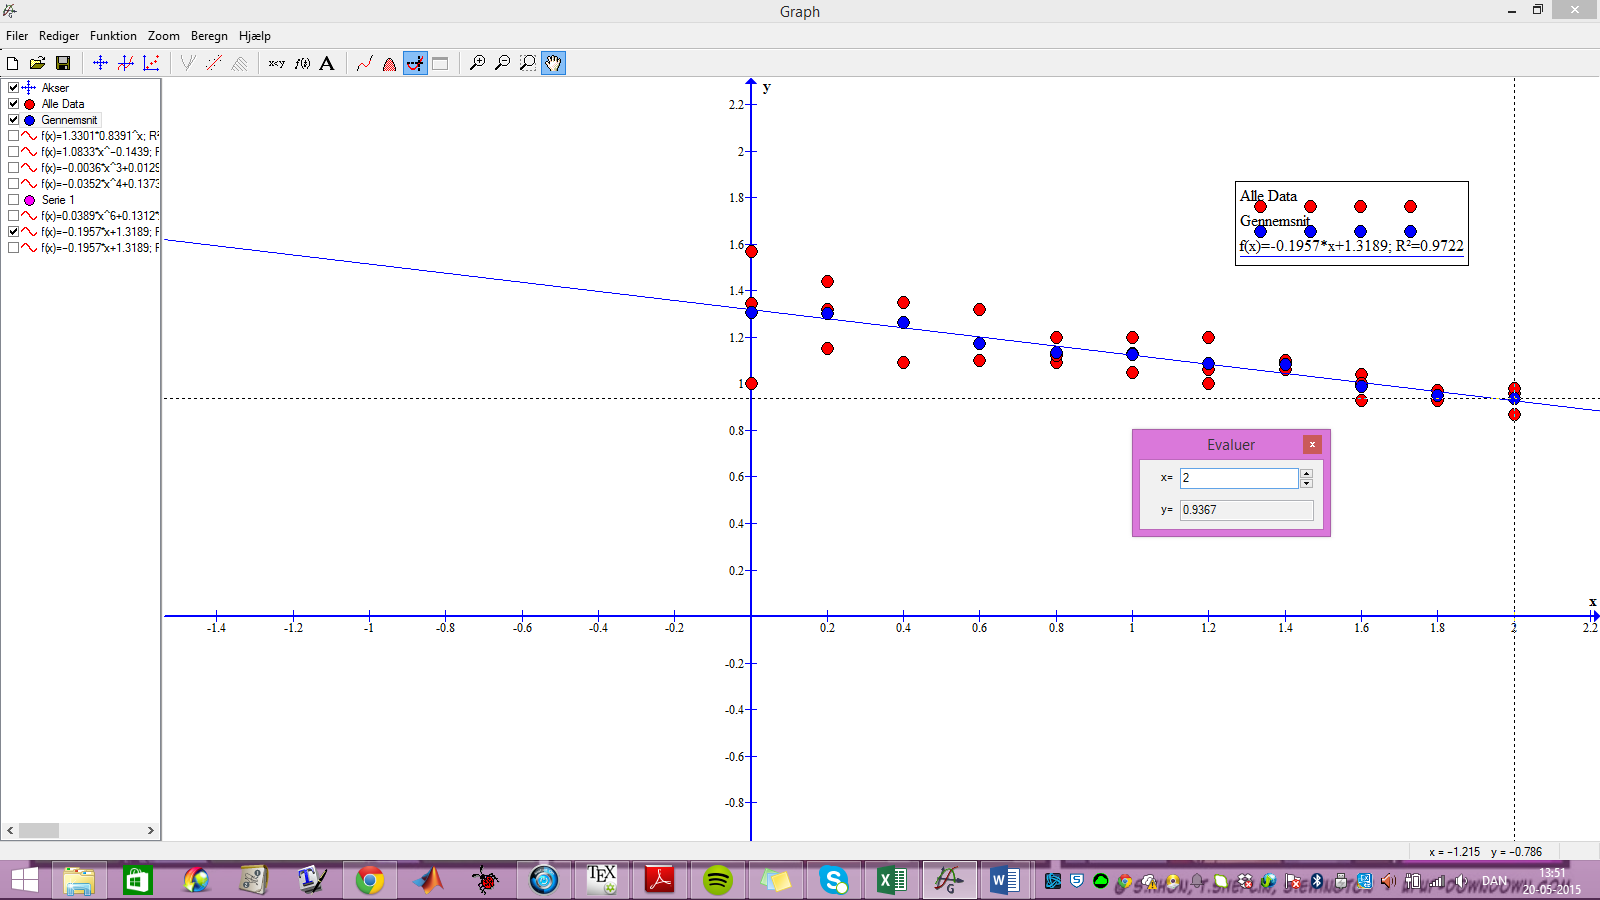
\includegraphics[scale=0.2]{./Graphics/Graf_Elektromagnet_resultater}
\caption{Data sættet i graf}
\label{Elektromagnet}
\end{figure}
Her ligger punkterne over data sættet, hvor de røde punkter er data for alle forsøgene og de blå er gennemsnittet af disse forsøg. Vi får nu at der er en kraft på 0.9367 N, ved luftgabet på 2 mm.

\subsubsection*{Udregninger}
Vi udregner hvordan elektromagneten ville virke under ideele forhold, det vil sige hvis, der ikke var nogen flux spredning i elektromagneten. For udregningerne begynder antages det at materialet er en negering af jern, som ligger mellem 300-500 relativ permeabilitet.\\

$H_{j}l_{j}+2H_{g}x=IN$ \\

$H_{j}=\frac{B_{j}}{\mu_{0}\mu_{r}},\,H_{g}=\frac{B_{g}
}{\mu_{0}}$\\

Ved at antage at der ikke er nogen spredning i luftgabet er $B_{g}=B_{j}$ som nu giver:\\

$\frac{B_{g}}{\mu_{0}\mu_{r}}*l_{j}+2*\frac{B_{g}}{\mu_{0}}=IN$\\



 
